% Preview source code

%% LyX 2.0.0 created this file.  For more info, see http://www.lyx.org/.
%% Do not edit unless you really know what you are doing.
\documentclass[a4paper,12pt,spanish]{article} %agregar twoside para impresion Doble Faz.
\usepackage[T1]{fontenc}
\usepackage{float}
\usepackage{amstext}
\usepackage{graphicx}
\usepackage[spanish, activeacute]{babel} %Paquetes para que funcionen bien los acentos.
\usepackage[utf8]{inputenc} 


\makeatletter

%%%%%%%%%%%%%%%%%%%%%%%%%%%%%% LyX specific LaTeX commands.
\newcommand{\lyxmathsym}[1]{\ifmmode\begingroup\def\b@ld{bold}
  \text{\ifx\math@version\b@ld\bfseries\fi#1}\endgroup\else#1\fi}


%%%%%%%%%%%%%%%%%%%%%%%%%%%%%% Textclass specific LaTeX commands.
\newenvironment{lyxlist}[1]
{\begin{list}{}
{\settowidth{\labelwidth}{#1}
 \setlength{\leftmargin}{\labelwidth}
 \addtolength{\leftmargin}{\labelsep}
 \renewcommand{\makelabel}[1]{##1\hfil}}}
{\end{list}}
\newenvironment{lyxcode}
{\par\begin{list}{}{
\setlength{\rightmargin}{\leftmargin}
\setlength{\listparindent}{0pt}% needed for AMS classes
\raggedright
\setlength{\itemsep}{0pt}
\setlength{\parsep}{0pt}
\normalfont\ttfamily}%
 \item[]}
{\end{list}}

\makeatother

\begin{document}

\title{Filesystems, IPCs y Servidores Concurrentes }

\maketitle

\section*{TP especial SO - 1}
\begin{lyxlist}{00.00.0000}
\item [{Integrantes:}]~\end{lyxlist}
\begin{enumerate}
\item Castiglione, Gonzalo - $49138$
\item Gomez, Horacio - $50825$
\item Orsay, Juan Pablo - $49373$
\end{enumerate}
\pagebreak{}


\section{Resumen}

Para este trabajo se pedía la realización de una simulación de empresas,
la cuales tienen aviones a su mando, encargados de distribuir sus
medicamentos por una serie de ciudades con conexiones entre ellas
limitadas.

\pagebreak{}


\section{Modelo}

Para llegar a la estructura de la simulación actual, primero se estudio
la diferencia entre procesos y threads. Los threads presentaban la
ventaja de ser $light$ $weight$ y que no necesitan comunicación
mediante un $IPC$ para pasarse información dado que corren en la
misma zona de código. Mientras que los procesos realizan una copia
de todas sus variables cuando son creados y corren independientes
de los cambios que el proceso padre haga. Teniendo estos detalles
en cuenta, se decidió que cada $Compania$ debía ser un proceso, ya
que no tiene porque compartir su información con nadie mas. Y, dado
que los aviones comparten todo con su empresa, nos resulto conveniente
optar por $Threads$ para estos.

Al tomar este tipo de estructura, surgió el problema sobre tipos de
mensajes entre estos procesos y cual era la forma óptima de comunicarlos
dado que el pasaje de información es mucho mas complejo que la comunicación
entre threads, ya que requiere tanto sincronización como una zona
de memoria ya preparada para la lectura y escritura. \\


Tomada esta decisión de diseño, se debía resolver además el problema
de:
\begin{enumerate}
\item Mostrar en pantalla los cambios de cada $Compania$ luego de cada
turno.
\item Reflejar en las demás companias los cambios producidos en el mapa
por la compaia $X$ antes que la compania $Y$ intente hacer un cambio
sin haber recibido esta notificación.\\

\end{enumerate}
La primer solución propuesta fue la de crear un zona de memoria compartida
la que involucraría tener en cuenta los siguientes aspectos:
\begin{itemize}
\item Todo aquel proceso que quisiese modificar esta zona de memoria, tendría
que hacerlo siempre bloqueando previamente un mutex (o semaforo en
su defecto) y luego de realizados los cambios liberar el mutex. Lo
cual obligaría a los demás procesos a {}``esperar'' en una cola
a acceder a esta memoria. El problema con esta implementación es que
si se hubiese implementado, no se se hubiese respetando la consigna
de usar los diferentes tipos de ipcs para la comunicación entre procesos.
Sin embargo es una solución agradable ya que evitaba el tener que
andar notificando a otras companias mediante paquetes especiales sobre
cambios realizados.
\end{itemize}
La segunda solución propuesta involucraba un proceso $servidor$
que se encargaría de la administración de turnos y recursos para cada
compania.
\begin{itemize}
\item Este presentaba la ventaja de tener una implementación muy sencilla
ya que solamente se ocuparía de levantar semáforos y bajarlos para
que las companias toquen el mapa en forma sincronizad y además asegurar
que ninguna valla a jugar dos veces seguidas (luego veremos que, como
en toda buena idea, trajo sus complicaciones).

\begin{itemize}
\item A su vez se podía saber cuando todas las companias habían terminado
un turno; por lo que actualizar la UI por turno resultaría muy sencillo.
\item La única contra que encontramos es que la comunicación con las companias
se volvia un tanto compleja.
\end{itemize}
\end{itemize}
\begin{figure}[H]
\hspace{1cm}\includegraphics[scale=0.5]{\string"Tp Diseno\string".png}

\caption{Estructura de procesos y threads de la simulación}


Al iniciar el programa, lo primero que se realiza es el parseo de
la información (de companias, mapas), inicialización del entorno (IPCs,
semáforos, handlers de las señales, inicialización de los nuevos procesos...)
y luego de terminado todo esto, se procede a inicializar el proceso
de UI/Servidor.
\end{figure}


Uno de los primeros (y mas grandes) problemas que se presentaron al
aplicar este diseño era de como reflejar los cambios hechos por una
compania en todas las demás. Inicialmente, se decidió que el servidor
tendría una (y la única) instancia del mapa y que se pasaría al principio
del turno a la compania, esta lo modificaria y luego se lo pasaría
nuevamente al servidor con los cambios. Y así para cada compania. 

Pero esta solución era muy costosa, ya que además de tener que mandar
el mapa, se debía mostrar por pantalla (en forma ordenada) toda la
información de la empresa; por lo que además de tener que pasar el
mapa dos veces, se tendría que sumar toda la compania, lo cual implicaría
muchísimo procesamiento y uso de memoria que podría ser ahorrado!.

Lo que nos llevo a proponer una segunda solución alternativa, la cual
implicaba que tanto el servidor como las companias tendrían una instancia
del mapa(inicial) y este se iría actualizando mediante paquetes $updates$
que se enviarian desde el servidor luego de cada turno. 

Esto presenta la ventaja que la comunicación entre los procesos se
reduciría a únicamente sus cambios! pero la contra esta en que requería
de una clase $serializer$ muchísimo mas completa que la que se tenia
en mente. Sin embargo, luego de discutirlo se llego a que se esta
era la mejor implementación %
\footnote{No se presentan calculos de cuanto mas se mejora dado que es muy fácil
notar la cantidad de información que se ahorra por cada envío de información%
}\\


Teniendo en cuenta todas estas consideraciones, la lógica del $servidor$
seguiría el siguiente comportamiento:

Por~cada~compania:
\begin{verbatim}
Se~le~da~un~turno.

Se~espera~a~que~finalize~su~turno.

Se~hace~un~broadcasting~de~los~updates~leidos~a~

~~~todas~las~demás~companias.

Actualizar~UI.~\\

\end{verbatim}
De esta manera, resulta fácil imaginar la lógica de una $compania$:
\begin{verbatim}
Despierto~a~todos~mis~aviones.

Cuando~todos~movieron,~actualizo~a~un~nuevo~target~a~todos

~~~~aquellos~que~llegaron~a~destino.

Escribo~los~paquetes~con~los~cámbios~realizados~por~cada~uno~al~servidor.

Me~escribo~a~mi~misma.
\end{verbatim}
A continuación de presenta un esquema de como se penso a una compania:

\begin{figure}[H]
\hspace{1cm}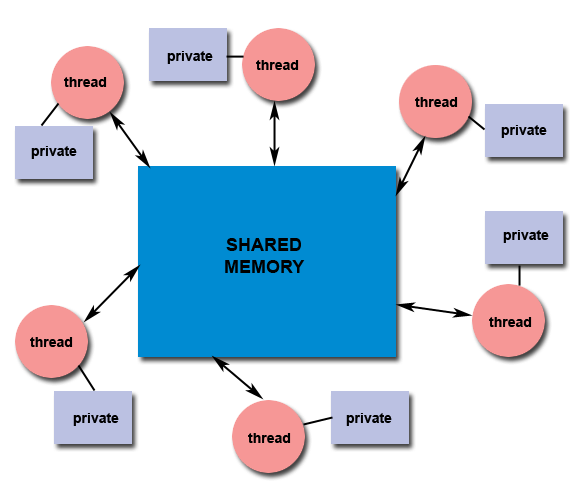
\includegraphics[scale=0.5]{airlineModl}

\caption{Esquma de una compania}
(figura tomada del sitio: http://www.chuidiang.com)
\end{figure}


Tal como se explico anteriormente, cada $Thread$ representa a un
avión activo, en donde este tiene su memoria propia (ítems, posición,
target, ...), una memoria compartida (el mapa) y un comportamiento.
Cuando un avion no tiene movimientos posibles, se mata al proceso,
y este ciclo sigue hasta que ningún avión tenga movimientos disponibles.
En cuyo caso se envia un paquete de tipo $company$ $status$ $update$
al servidor y se encargara de hacer lo que sea necesario.

\pagebreak{}


\section{IPC}

Al principio se comenzó experimentando comunicación entre procesos
con pipes. Luego de varias complicaciones de llego a una primera versión
de metodos de IPC formada por diversos metodos. Esta nos sirvió como
base para ir experimentando como funcionaban los semáforos y mutex
en linux. Luego, a medida que el programa iba tomando forma y sentido,
se comenzó a mejorarla y se implementó $Fifos$, $MsgQueues$, $Sockets$
y $Shared$ $Memory$.

Uno de los mayores inconvenientes al momento de implementación de
los IPCS era la sincronización, ya que, por mas pruebas que se les
halla a cada antes de ser montados al código de la simulación, se tenia
el problema que cuando no se leía en forma ordenada, este decía que
no había mensajes cuando se esperaba que los hubiera, lo que llevaba
a mucha perdida de tiempo en debugeo de código.

Una de las complicaciones que tuvimos con los IPCs era el tamaño de
los datos a escribir, dado que para algunos IPCs era mas fácil trabajar
con tamaños fijos y con otros daba igual, se opto por paquetes de
tamaño fijo. Esto facilitó mucho la programación de la interfaz de
comunicación, pero tiene el problema importante que si se quiere serializar
una gran compania con muchos aviones e ítems, puede resultar que este
string serializado resultante sea mas largo que el tamaño default.
Lo que provocaria que el paquete no se mande y quede inconsistente
el resultado de la simulación. 

De todas maneras, si esto llegase a suceder, un mensaje de error se
mostrara en el $log.txt$. En cuyo caso lo único que se tiene que
arreglar es el $DATA$\_$SIZE$ definido en $communicator.h$.

Otro inconveniente que trae esta decisión que tamaño fijo para mensajes
es el desperdicio de memoria innecesario por ejemplo para mandar un
pequeño update. Sin embargo, no es un gran problema, si el dia de
mañana se necesitase que esto no sea así, bastara con simplemente
cambiar la implementación del IPC correspondiente (no afectaría de
ninguna manera a la simulación).\\



\subsection{Shared Memory}

La implementación que actualmente se tiene para shared memory, es
aprovechar el hecho que los tamaños de los mensajes son fijos y reservar
en memoria bloques con un tamaño de $M$ mensajes por cada proceso
que quiera escribir. Es decir, dividimos un pedazo fijo de memoria
en $NxN$ lugares, en donde $N$ esta dado por la cantidad de lugares
especificados en $ipc$\_$init$. Esta implementación ofrece la ventaja
de ser muy eficiente en cuando acceso a un mensaje, ya que tiene una
complejidad $o(1)$, pero la gran contra es que es mucha la memoria
que necesita tener reservada.

Dentro de cada lugar de esta matriz, se tiene un array con los $M$
lugares ya mencionados y adelante de todo un $char$ indicando cuantos
se tienen en la lista.


\subsection{Típos de paquetes}

Actualmente la comunicación entre $servidor\Longleftrightarrow compania$
se realiza mediante tres tipos de paquetes:\\

\begin{itemize}
\item City update: Este paquete contiene información de que ítem fue modificado
en que ciudad y en que cantidad. Si muchas ciudades fueron modificadas
en un turno, uno por cada cambio va a ser enviado al servidor.
\item City status update: Este paquete se envia cuando una compania detecto
que sus aviones no pueden abastecer a mas ciudades y quiere {}``darse
de baja'' en el servidor. Es importante esto ya que, una vez que
una compania se desactiva en el servidor, automáticamente se deja de
encolarle actualizaciones. Lo que resulta es un ahorro importante
en llamadas al serializer y de uso de recursos del IPC para mantener
mensajes que nunca serial leídos.
\item Company update: este es el paquete mas grande que se tiene, aqui es
donde se guarda la información de todos los aviones que tiene una
compania. El problema es que crece mucho a medida que se agregan mas
items y/o aviones la misma. Por lo que quedaria en el $"wish$ $list"$,
partir este paquete en otros mas pequeños y en lo posible con tamaño
constante, para de esta manera poder reducir el DATA\_SIZE que se
necesita tener reservado para usar el IPC. Que en estos momentos seria
lo que mas recursos consume de la simulación. Se tenia pensando para
estos, realizar lo mismo que para las ciudades, solamente mandar pequeños
paquetes updates en vez de repetir una y otra vez la misma información
que no sufrió cambios.
\end{itemize}
\pagebreak{}


\section{Otras consideraciones}

Uno de los problemas mas difíciles que constantemente se presentaba
durante el desarrollo del trabajo era sobre la dura elección entre
$tiempo$ $vs$ $memoria$. Si se debía hacer cierto calculo al momento
de necesitarlo o bien guardarlo previamente y simplemente actualizarlo
cuando sea necesario.

Al principio, cada vez que un avión llegaba a una ciudad, se realizaba
un DFS para encontrar el camino a las ciudad mas corta que sea abastecible.
El problema es que este mismo DFS se estaba realizando por cada avión,
por cada compania en cada turno. Lo que nos parecia que se realizaba
el mismo calculo innecesariamente muchísimas veces. Por lo que se
propuso una matriz en donde, por cada compania se colocaria un indice
diciendo a donde hay que ir para acceder a la ciudad $X$ (para cualquier
ciudad) y a que distancia se encuentra. Esto reduciría la llamada al
$DFS$ a desrefenciar una matriz ($o(1)$), esta fue una de las luchas
mencionadas anteriormente, sobre la utilización de memoria espacial
o de tiempo%
\footnote{Esta razón de necesitar implementar un DFS surgió en casos cuando
solo se podia abastecer a una ciudad que no era adyacente a la posición
actual del avión.%
}.

Otro cambio de la misma índole que se propuso durante la realización
del trabajo es que cada ID de un elemento representaba a la posición
en el array que ocuparía. Es decir, el elemento con Id $5$, se lo
encontraria en el array de elementos en la quinta posición. Esto trae
consecuencias como tener un array de $20$ elementos solo para tener
un elemento con ID $20$. Sin embargo, para la búsqueda de items (la
cual se realiza constantemente) reduce un algoritmo de $o(n)$ a uno
de $o(1)$ con el precia de agregar un extra en la cantidad de memoria
necesaria para su funcionamiento.

Se tuvo un problema de ultimo momento con dos de los $IPCs$ (Sockets
y Fifos) que dejaron de andar y se trataron de arreglar pero no se
pudo testear si verdaderamente tienen una funcionalidad $100\%$ correcta. 

El problema con sockets es que era necesario mantener una referencia al file 
descriptor del socket de lectura y eso no lo descubrimos hasta ultimo momento.
Nos hubiese dado mucho gusto encontrar la solución  de esto pero nos quedamos 
sin tiempo para la entrega. Por lo que se tuvo que 
implementar un array de tamaño fijo para almacenar estos files descriptos.
Queda en la lista arreglar eso y hacerlo independiente de la implementacion.


\subsection{Otras problemas}

Un problema al que todavía no pudimos encontrar explicación es porque
los semáforos de $System$ $V$ a veces no se inicializaban para ciertos
valores de claves. Se intento eliminarlos, cambiar los flags de creacion,
reiniciar la comutadora pero todo sin suerte! Mas raro resultaba aun
que al sumarle un magic number al key, éstos se creban y sin problema.
Por lo que nuestra única alternativa fue la de pasar a semáforos de
Posix. Los cuales resultaron increiblemente mas simples. Lo mismo
sucede a veces con la creación de los $IPCs$, que a veces no logran
cerrarse correctamente al finalizar el programa o bien el recuso del
SO se encuentra ocupado y se rehusa a crear los IPS terminando en
resultados sin sentido, por lo que se recomienda que si esto sucede
se utilize el comando $ipcs$ para verificar que no se tenga una excesiva
cantidad de estos andando (se soluciona también reiniciando ya que
para todo tipo de almacenamiento temporal, se utiliza la carpeta $/tmp$
del SO.

Se quería aclarar que si se testea la simulación de archivos que tienen
formatos invalidos, el programa resultara en $segmentation$ $fault$.
Esto no fue arreglado ya que supusimos que lo importante de este trabajo
practico no era ver quien hacia el parser mas robusto sino el de demostrar
el poder del uso de IPCs. Por lo que se recomienda verificar bien
el formato de los archivos antes de iniciar el programa.

\pagebreak{}


\section{Concusiones}

Luego de realizado este trabajo practico, se aprendió sobre la potencia
a la que se puede llevar un programa al hacerlos que sean capaces
de dividir sus tareas en procesos concretos y por sobre todo, al mantenerlos
sincronizados. 
Existen diferentes formas para comunicar procesos:
\begin{itemize}
 \item socket: es el único que permite sincronización entre diferentes máquinas. También
utilizan archivos especiales del tipo socket para trabajar localmente.
 \item shared memory: es veloz y mucho más difícil de implementar, hay que manejar la
memoria a mano y a menos que se utilicen librerías como $OSSP mm$ (Shared Memory Allocation)
no se puede alocar memoria (malloc) dentro del segmento compartido.
 \item fifo: crea tipos especiales de archivo en el filesystem también conocidos como
''named pipes'', de fácil utilización.
 \item msg queue: similar a fifo, utiliza colas para almacenar mensajes con keys para
acceder a ellas.
\end{itemize}
Es necesario sin embargo manejar la sincronización de los mencionados ipc para que los
diferentes procesos que acceden a ellos no dejen inconsistencias en la comunicación.


\end{document}

